% The parameter plane is zeta_0+zeta_1+zeta_2=0.
% This drawing uses zeta_0=x, zeta_1=-x/2-sqrt(3)y/2,
% zeta_2=-x/2+sqrt(3)y/2. It is not the (s,t) coordinate plane.
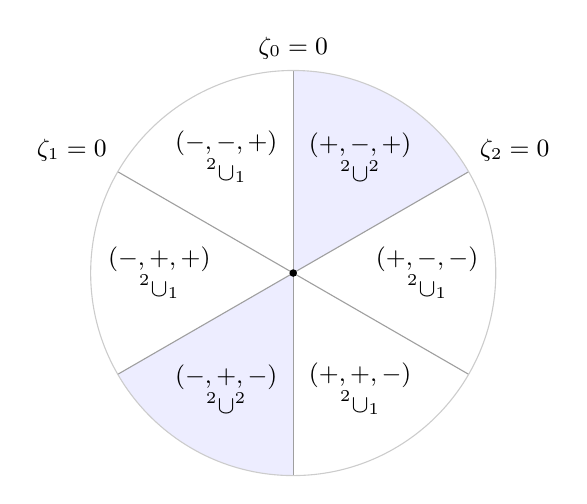
\begin{tikzpicture}[scale=1.05,font=\small]
 \fill[blue!7] (0,0)--(30:2.45) arc(30:90:2.45)--cycle;
 \fill[blue!7] (0,0)--(210:2.45) arc(210:270:2.45)--cycle;
 \foreach \angle in {30,90,150}
  {\draw[gray!75] (\angle:2.45)--(\angle+180:2.45);}
 \draw[gray!40] (0,0) circle[radius=2.45];
 \fill (0,0) circle[radius=1.3pt];
 \node[align=center] at (0:1.62) {$(+,-,-)$\\$\PP^2\cup\FF_1$};
 \node[align=center] at (60:1.62) {$(+,-,+)$\\$\PP^2\cup\PP^2$};
 \node[align=center] at (120:1.62) {$(-,-,+)$\\$\PP^2\cup\FF_1$};
 \node[align=center] at (180:1.62) {$(-,+,+)$\\$\PP^2\cup\FF_1$};
 \node[align=center] at (240:1.62) {$(-,+,-)$\\$\PP^2\cup\PP^2$};
 \node[align=center] at (300:1.62) {$(+,+,-)$\\$\PP^2\cup\FF_1$};
 \node[above] at (90:2.47) {$\zeta_0=0$};
 \node[above right] at (30:2.47) {$\zeta_2=0$};
 \node[above left] at (150:2.47) {$\zeta_1=0$};
\end{tikzpicture}
